% Author: Izaak Neutelings (June 2020)
% Inspiration:
%  https://courses.physics.ucsd.edu/2011/Summer/session1/physics2c/diffraction.pdf
%  https://tex.stackexchange.com/questions/201830/periodic-shading-in-tikz
\documentclass[border=3pt,tikz]{standalone}
\usepackage[outline]{contour} % glow around text
\usepackage{physics}
\usepackage{xcolor}
\usepackage{etoolbox} %ifthen
\usetikzlibrary{calc}
\usetikzlibrary{arrows,arrows.meta}
\usetikzlibrary{decorations.markings}
\usetikzlibrary{angles,quotes} % for pic (angle labels)
\usetikzlibrary{fadings}
\tikzset{>=latex} % for LaTeX arrow head
\contourlength{1.4pt}

\colorlet{wall}{blue!30!black}
\colorlet{myblue}{blue!70!black}
\colorlet{myred}{red!70!black}
\colorlet{mydarkred}{red!50!black}
\colorlet{mylightgreen}{green!60!black!70}
\colorlet{mygreen}{green!60!black}
\colorlet{myredgrey}{red!50!black!80}
\colorlet{myshadow}{blue!30!black!90}
\tikzstyle{wave}=[myblue,thick]
\tikzstyle{mydashed}=[black!70,dashed,thin]
\tikzstyle{mymeas}=[{Latex[length=3,width=2]}-{Latex[length=3,width=2]},thin]
\tikzstyle{mysmallarr}=[-{Latex[length=3,width=2]}]


\newcommand\rightAngle[4]{
  \pgfmathanglebetweenpoints{\pgfpointanchor{#2}{center}}{\pgfpointanchor{#3}{center}}
  \coordinate (tmpRA) at ($(#2)+(\pgfmathresult+45:#4)$);
  \draw[white,line width=0.6] ($(#2)!(tmpRA)!(#1)$) -- (tmpRA) -- ($(#2)!(tmpRA)!(#3)$);
  \draw[mydarkred] ($(#2)!(tmpRA)!(#1)$) -- (tmpRA) -- ($(#2)!(tmpRA)!(#3)$);
}
\newcommand\lineend[2]{
  \def\w{0.1} \def\c{30}
  \draw[mygreen] (#1)++(#2:\w) to[out=#2-180-\c,in=#2+\c] (#1)
                               to[out=#2+\c-180,in=#2-\c]++ (#2-180:\w);
}
\def\tick#1#2{\draw[thick] (#1) ++ (#2:0.1) --++ (#2-180:0.2)}

% INTERFERENCE FADING
\begin{tikzfadingfrompicture}[name=interference]
  \def\lambd{0.5} % wavelength
  \foreach \r in {1,...,15}
    \foreach \j in {1,...,25}
       \path [line width=\lambd*\j,draw=transparent!0,opacity=0.04]
          (0,0) circle (\lambd*\r); %(0:\r) arc (0:180:\r);
\end{tikzfadingfrompicture}



\begin{document}


% INTERFERENCE FADING
\begin{tikzpicture}
  \def\a{2}  % distance sources
  \def\W{8} % distance between walls
  \def\H{8}  % total wall height
  %\clip (-\W/2,0) rectangle ++(\W,\H);
  \path[fill=myshadow,path fading=interference,fit fading=false,fading transform={shift={(0,\a/2)}}] %,shift={(-2,0)}
    (0,-\H/2) rectangle ++(\W,\H);
  \path[fill=myshadow,path fading=interference,fit fading=false,fading transform={shift={(0,-\a/2)}}] %rotate=45
    (0,-\H/2) rectangle ++(\W,\H);
  %\draw (0,0) --++ (0,\H);
\end{tikzpicture}


% TWO SPLIT
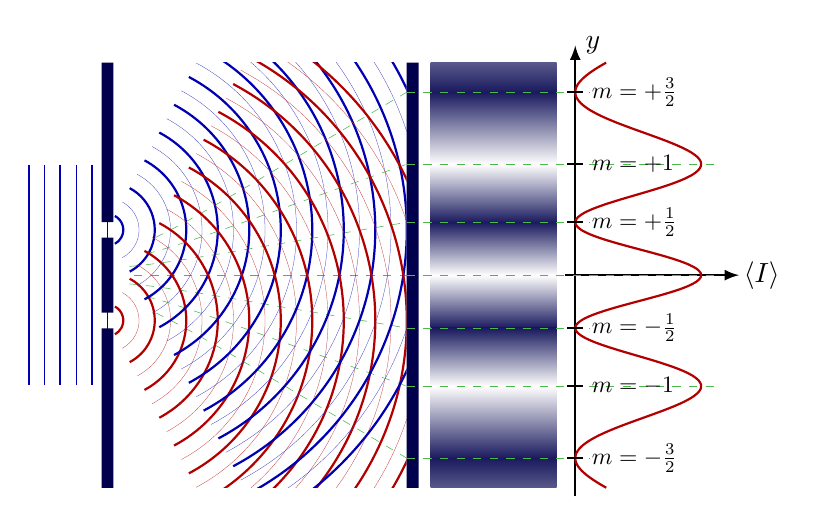
\begin{tikzpicture}[
    nodal/.style={mylightgreen,dashed,very thin},
    declare function={
      %xnode(\n,\dn,\lam,\f) = sqrt( (\n^2+(\n+\dn)^2)*\lambd^2/2 - (\n^2-(\n+\dn)^2)^2*\lambd^4/(4*\a^2) - \a^2/4 );
      xnode(\n,\dn,\lam,\f) = \lam/\f*sqrt( \n^2*(\f^2-\dn^2)+\n*\dn*(\f^2-\dn^2)+\dn^2*\f^2/2-(\f^4+\dn^4)/4 );
      ynode(\n,\dn,\lam,\a) = (2*\n*\dn+\dn^2)*\lam/(2*\f);
      intensity(\y,\lam,\a,\L) = cos(180*\a*\y/(2*\lam*sqrt(\L*\L+\y*\y)))^2;
    }
  ]
  
  \def\L{3.8}       % distance between walls
  \def\H{5.4}       % total wall height
  \def\h{2.8}       % plane wave height
  \def\t{0.15}      % wall thickness
  \def\a{1.15}      % slit distance
  \def\d{0.20}      % slit size
  \def\N{21}        % number of waves
  \def\lambd{0.20}  % wavelength
  \def\R{\N*\lambd} % wave radius
  \def\Nlines{3}    % number of nodal lines
  \def\A{1.6}       % amplitude
  %\def\r{0.06}      % point source radius
  %\def\nmax{10}
  \def\nsamples{100}
  \def\ang{62}
  
  \begin{scope}
    \clip (-\t/2,-\H/2) rectangle (\L,\H/2);
    %\clip (-\t/2,0.7*\a) -- (0.6*\L,\H/2) -- (\L,\H/2) --
    %      (\L,-\H/2) -- (0.6*\L,-\H/2) -- (-\t/2,-0.7*\a) -- cycle;
    
    % NODAL LINES
    \draw[nodal]
      (0.08*\N*\lambd,0) -- (1.06*\R,0);
    \coordinate (NP0) at (\L,0);  % to avoid "Dimension too large error"
    \foreach \dn [evaluate={
                   \f=\a/\lambd;
                   \nmin=2.5+0.2*\dn; %0.501*(-\dn+\f)
                   \nmax=10; %(NP0)
                   \c=int(\dn<\f);
                   \y=\L/sqrt((\a/(\lambd*\dn))^2-1);
                 }] in {1,...,\Nlines}{
      \coordinate (NP+\dn) at (\L,\y);  % to avoid "Dimension too large error"
      \coordinate (NP-\dn) at (\L,-\y); % to avoid "Dimension too large error"
      \ifnum\c=1
        \draw[nodal,variable=\n,samples=\nsamples,smooth]
          plot[domain=\nmin:\nmax] ({xnode(\n,\dn,\lambd,\f)},{ynode(\n,\dn,\lambd,\f)})
          -- (NP+\dn);
        \draw[nodal,variable=\n,samples=\nsamples,smooth]
          plot[domain=\nmin:\nmax] ({xnode(\n,\dn,\lambd,\f)},{-ynode(\n,\dn,\lambd,\f)})
          -- (NP-\dn);
      \fi
    }
    
    % WAVES
    \foreach \i [evaluate={\R=\i*\lambd;}] in {1,...,\N}{
      \ifodd\i
        \draw[myblue,line width=0.8] (0,\a/2)++(\ang:\R) arc (\ang:-\ang:\R);
        \draw[myred,line width=0.8] (0,-\a/2)++(\ang:\R) arc (\ang:-\ang:\R);
      \else
        \draw[myblue!80,line width=0.1] (0,\a/2)++(\ang:\R) arc (\ang:-\ang:\R);
        \draw[myred!80,line width=0.1] (0,-\a/2)++(\ang:\R) arc (\ang:-\ang:\R);
      \fi
    }
  \end{scope}
  
  % PLANE WAVES
  \foreach \i [evaluate={\x=-\i*\lambd;}] in {0,...,5}{
    \ifodd\i
      \draw[myblue,line width=0.8] (\x,-\h/2) -- (\x,\h/2);
    \else
      \draw[myblue,line width=0.1] (\x,-\h/2) -- (\x,\h/2);
    \fi
  }
  
  % WALL
  \fill[wall]
    (\t/2,\a/2-\d/2) rectangle (-\t/2,-\a/2+\d/2)
    (\t/2,\a/2+\d/2) rectangle (-\t/2,\H/2)
    (\t/2,-\a/2-\d/2) rectangle (-\t/2,-\H/2)
    (\L,-\H/2) rectangle (\L+\t,\H/2);
  
  % SHADES
  \begin{scope}[shift={(1.08*\L,0)}]
    \def\yz{\L/sqrt((\a/\lambd)^2-1)} % m = +- 1/2
    \def\yZ{\L/sqrt((\a/\lambd/2)^2-1)} % m = +- 1
    \clip (0,-\H/2) rectangle (1.1*\A,\H/2);
    \fill[white] (0,-\H/2) rectangle++ (\A,\H); % to fill seams
    \foreach \i [evaluate={\n=0.5*\i;\yn=\L/sqrt((\a/(2*\lambd*\n))^2-1);
                 }] in {1,...,\Nlines}{
      \ifodd\i % if even
        \fill[myshadow] (0,{-\yn-0.1}) rectangle++ (\A,0.2); % to fill seams
        \fill[myshadow] (0,{ \yn-0.1}) rectangle++ (\A,0.2); % to fill seams
      \fi
    }
    \path[left color=myshadow,right color=myshadow,middle color=white,shading angle={180}]
      (0,{-\yz}) rectangle (\A,{\yz});
    \foreach \i [evaluate={
                  \n=0.5*\i;
                  \m=0.5*(\i+1);
                  \yn=\L/sqrt((\a/(2*\lambd*\n))^2-1);
                  \ym=\L/sqrt((\a/(2*\lambd*\m))^2-1);
                  \dang=mod(\i,2)*180;
                 }] in {1,...,\Nlines}{
      \path[left color=myshadow,right color=white,shading angle={\dang}]
        (0,\yn) rectangle (\A,\ym);
      \path[left color=myshadow,right color=white,shading angle={180+\dang}]
        (0,-\yn) rectangle (\A,-\ym);
    }
  \end{scope}
  
  % INTENSITY
  \begin{scope}[shift={(1.1*\L+1.1*\A,0)}]
    \draw[->,thick] (-0.08*\A,0) -- (1.3*\A,0) node[right=-2] {$\expval{I}$}; % I axis
    \draw[->,thick] (0,-0.52*\H) -- (0,0.54*\H) node[right] {$y$}; % y axis
    \draw[nodal] (NP0) --++ (0.15*\L+2.1*\A,0); % green nodal lines
    \foreach \i [evaluate={\y=\L/sqrt((\a/(\lambd*\i))^2-1)}] in {1,...,\Nlines}{ % green nodal lines
      \draw[nodal] (NP+\i) --++ ({0.15*\L+1.1*\A+\A*intensity(\y,\lambd,\a,\L)},0);
      \draw[nodal] (NP-\i) --++ ({0.15*\L+1.1*\A+\A*intensity(\y,\lambd,\a,\L)},0);
    }
    \draw[myred,thick,variable=\y,samples=\nsamples,smooth,domain=-\H/2:\H/2]
      plot({\A*intensity(\y,\lambd,\a,\L)},\y);
    \foreach \i [evaluate={ % ticks
        \modd=\i; %int(\i);
        \meven=int(\i-1);
        \y=\L/sqrt((\a/(\lambd*\i))^2-1);
                }] in {1,...,\Nlines}{
      \ifodd\i
        \tick{0,-\y}{180} node[right=0,scale=0.85] {$m=-\frac{\modd}{2}$};
        \tick{0,\y}{180} node[right=0,scale=0.85] {$m=+\frac{\modd}{2}$};
      \else
        \tick{0,-\y}{180} node[right=0,scale=0.85] {$m=-\meven$};
        \tick{0,\y}{180} node[right=0,scale=0.85] {$m=+\meven$};
      \fi
    }
  \end{scope}
  
\end{tikzpicture}


% TWO SLIT PATH DIFFERENCE
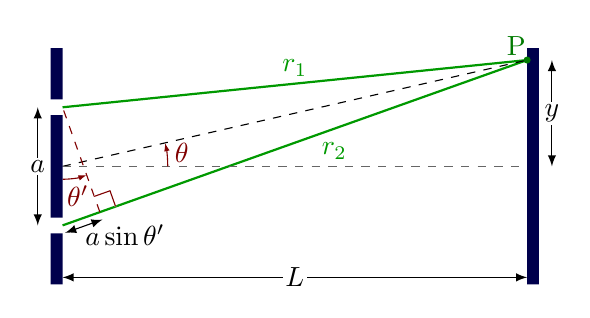
\begin{tikzpicture}
  
  \def\L{5.9}       % distance between walls
  \def\H{3.0}       % total wall height
  \def\f{0.9}       % fractional height of projection point
  \def\ang{atan((\f*\H+\a)/\L/2)} % theta
  \def\t{0.15}      % wall thickness
  \def\a{1.5}       % slit distance
  \def\d{0.20}      % slit size
  \coordinate (T) at (0,\a/2);
  \coordinate (B) at (0,-\a/2);
  \coordinate (L) at (0,0);
  \coordinate (R) at (\L,0);
  \coordinate (P) at (\L,\f*\H/2);
  \coordinate (M) at ($(B)!(T)!(P)$);
  
  % LINES
  \draw[mygreen,thick] (T) -- (P) node[midway,above=-1] {$r_1$};
  \draw[mygreen,thick] (B) -- (P) node[midway,below=3,right=6] {$r_2$}; %right=6,below right=-4
  \draw[dashed] (L) -- (P);
  \draw[dashed,black!60] (L) -- (R);
  \draw[mydarkred,dashed] (M) -- (T);
  
  % ANGLES
  \draw pic[mysmallarr,"$\theta'$",mydarkred,draw=mydarkred,angle radius=26,angle eccentricity=1.25]
    {angle = B--T--M};
  \draw pic[mysmallarr,"$\theta$",mydarkred,draw=mydarkred,angle radius=38,angle eccentricity=1.14]
    {angle = R--L--P};
  \rightAngle{T}{M}{P}{0.3}
  
  % MEASURES
  \draw[<->,black] (0,-0.47*\H) --++ (\L,0) node[midway,fill=white,inner sep=1] {$L$};
  \draw[<->,black] (-2.1*\t,-\a/2) --++ (0,\a) node[midway,fill=white,inner sep=1] {$a$};
  \draw[<->,black] ([shift={({\ang-90}:0.1)}]B) -- ([shift={({\ang-90}:0.1)}]M)
    node[midway,above=1,below right=-3]{$a\sin\theta'$};
  \draw[<->,black] ([shift={(2.1*\t,0)}]P) -- ([shift={(2.1*\t,0)}]R)
    node[midway,fill=white,inner sep=1]{$y$};
  
  % WALL
  \fill[wall]
    (0,\a/2-\d/2) rectangle (-\t,-\a/2+\d/2)
    (0,\a/2+\d/2) rectangle (-\t,\H/2)
    (0,-\a/2-\d/2) rectangle (-\t,-\H/2)
    (\L,-\H/2) rectangle (\L+\t,\H/2);
  \fill[mygreen!80!black] (P) circle (0.3*\t) node[right=1,above left=-2] {P};
  
\end{tikzpicture}


% TWO SLIT PATH DIFFERENCE close up
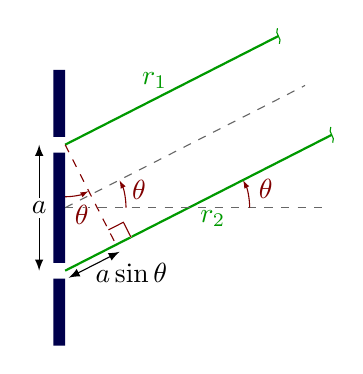
\begin{tikzpicture}
  
  \def\L{5.5}       % distance between walls
  \def\l{3.8}       % distance between walls
  \def\H{3.5}       % total wall height
  \def\f{0.9}       % fractional height of projection point
  \def\t{0.15}      % wall thickness
  \def\a{1.6}       % slit distance
  \def\d{0.20}      % slit size
  \def\ang{27}      % angle
  \coordinate (T) at (0,\a/2);
  \coordinate (B) at (0,-\a/2);
  \coordinate (L) at (0,0);
  \coordinate (R) at (\L,0);
  \coordinate (I) at ({\a/2/tan(\ang)},0);
  
  % LINES
  \draw[mygreen,thick] (T) --++ (\ang:.8*\l) coordinate (PT) node[midway,below=1,above left=-2] {$r_1$};
  \draw[mygreen,thick] (B) --++ (\ang:\l) coordinate (PB) node[midway,left=2,below right=-1] {$r_2$};
  \draw[mydarkred,dashed] (T) -- ($(B)!(T)!(PB)$) coordinate (M);
  \draw[black!60,dashed] (L) --++ (\ang:.9*\l) coordinate (PR);
  %\draw[black!60,dashed] (T) --++ (.20*\L,0) coordinate (TR);
  \draw[black!60,dashed] (L) --++ (.6*\L,0) coordinate (LR);
  %\draw[black!60,dashed] (B) --++ (.20*\L,0) coordinate (BR);
  
  % LINE END
  \lineend{PT}{\ang+70}
  \lineend{PB}{\ang+70}
  
  % ANGLES
  \draw pic[mysmallarr,"\contour{white}{$\theta$}",mydarkred,draw=mydarkred,angle radius=18.8,angle eccentricity=1.38 ]
    {angle = B--T--M};
  %\draw pic[->,"$\theta$",mydarkred,draw=mydarkred,angle radius=16,angle eccentricity=1.41]
  %  {angle = TR--T--PT};
  %\draw pic[->,"$\theta$",mydarkred,draw=mydarkred,angle radius=16,angle eccentricity=1.41]
  %  {angle = BR--B--PB};
  \draw pic[mysmallarr,"$\theta$",mydarkred,draw=mydarkred,angle radius=22,angle eccentricity=1.25]
    {angle = LR--L--PR};
  \draw pic[mysmallarr,"$\theta$",mydarkred,draw=mydarkred,angle radius=22,angle eccentricity=1.30]
    {angle = LR--I--PB};
  \rightAngle{T}{M}{PB}{0.3}
  
  % MEASURES
  \draw[<->,black] (-2.2*\t,-\a/2) --++ (0,\a) node[midway,fill=white,inner sep=1.5] {$a$};
  \draw[<->,black] ([shift={({\ang-90}:0.1)}]B) -- ([shift={({\ang-90}:0.1)}]M)
    node[midway,above=1,below right=-3]{$a\sin\theta$};
  
  % WALL
  \fill[wall]
    (0,\a/2-\d/2) rectangle (-\t,-\a/2+\d/2)
    (0,\a/2+\d/2) rectangle (-\t,\H/2)
    (0,-\a/2-\d/2) rectangle (-\t,-\H/2);
  
\end{tikzpicture}


\end{document}